\documentclass[10pt]{beamer}

\usepackage[utf8]{inputenc}
\usepackage[german]{babel}
\usepackage{amsmath}
\usepackage{amsfonts}
\usepackage{amssymb}
\usepackage{tikz}
\usepackage{enumitem}
\usepackage{listings}
\usepackage{xcolor}
\usepackage[german,lined]{algorithm2e}
\usepackage{float}

\usetheme{Rochester}
\useinnertheme{rectangles}
\useoutertheme{default}

\lstset{
	basicstyle=\small\ttfamily,
	keywordstyle=\color{blue},
	showstringspaces=true}

\title{Entwicklung eines Treibers und Toolchain zur Administration eines Embedded ZPU-Systems}
\author{
\includegraphics[width=0.5\textwidth]{images/hs_os}\\\vspace{0.5cm}
Oliver Erxleben\\Martin Helmich}
%\institute{Hochschule Osnabrück}
\date{27. Februar 2013}

\setitemize{label=\usebeamerfont*{itemize item}%
  \usebeamercolor[fg]{itemize item}
  \usebeamertemplate{itemize item}}

\begin{document}
    \thispagestyle{empty}
	\frame{\titlepage}
	
	\begin{frame}{Aufbau der Hardware}
		\begin{center}
		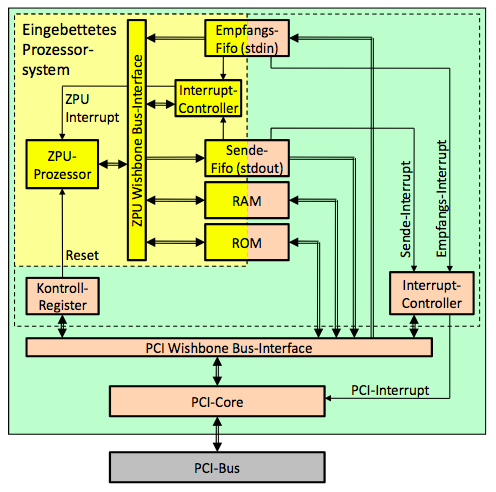
\includegraphics[height=0.9\textheight]{images/zpu_architecture.png}
		\end{center}
	\end{frame}
	
	\begin{frame}{Aufgabenstellung}
		\begin{itemize}
			\item \textbf{Zurücksetzen} des Prozessorsystems per \texttt{ioctl}-Befehl
			\item Einblenden des RAMs in den Userspace-Speicher per \texttt{mmap}, um \textbf{neue Software} in das System laden zu können.
			\item Senden von Eingaben an den \textbf{stdin}-Buffer und Lesen von Ausgaben aus dem \textbf{stdout}-Buffer per \texttt{read}- und \texttt{write}-Methoden.
		\end{itemize}
	\end{frame}
	
	\begin{frame}{Register der Hardware}
		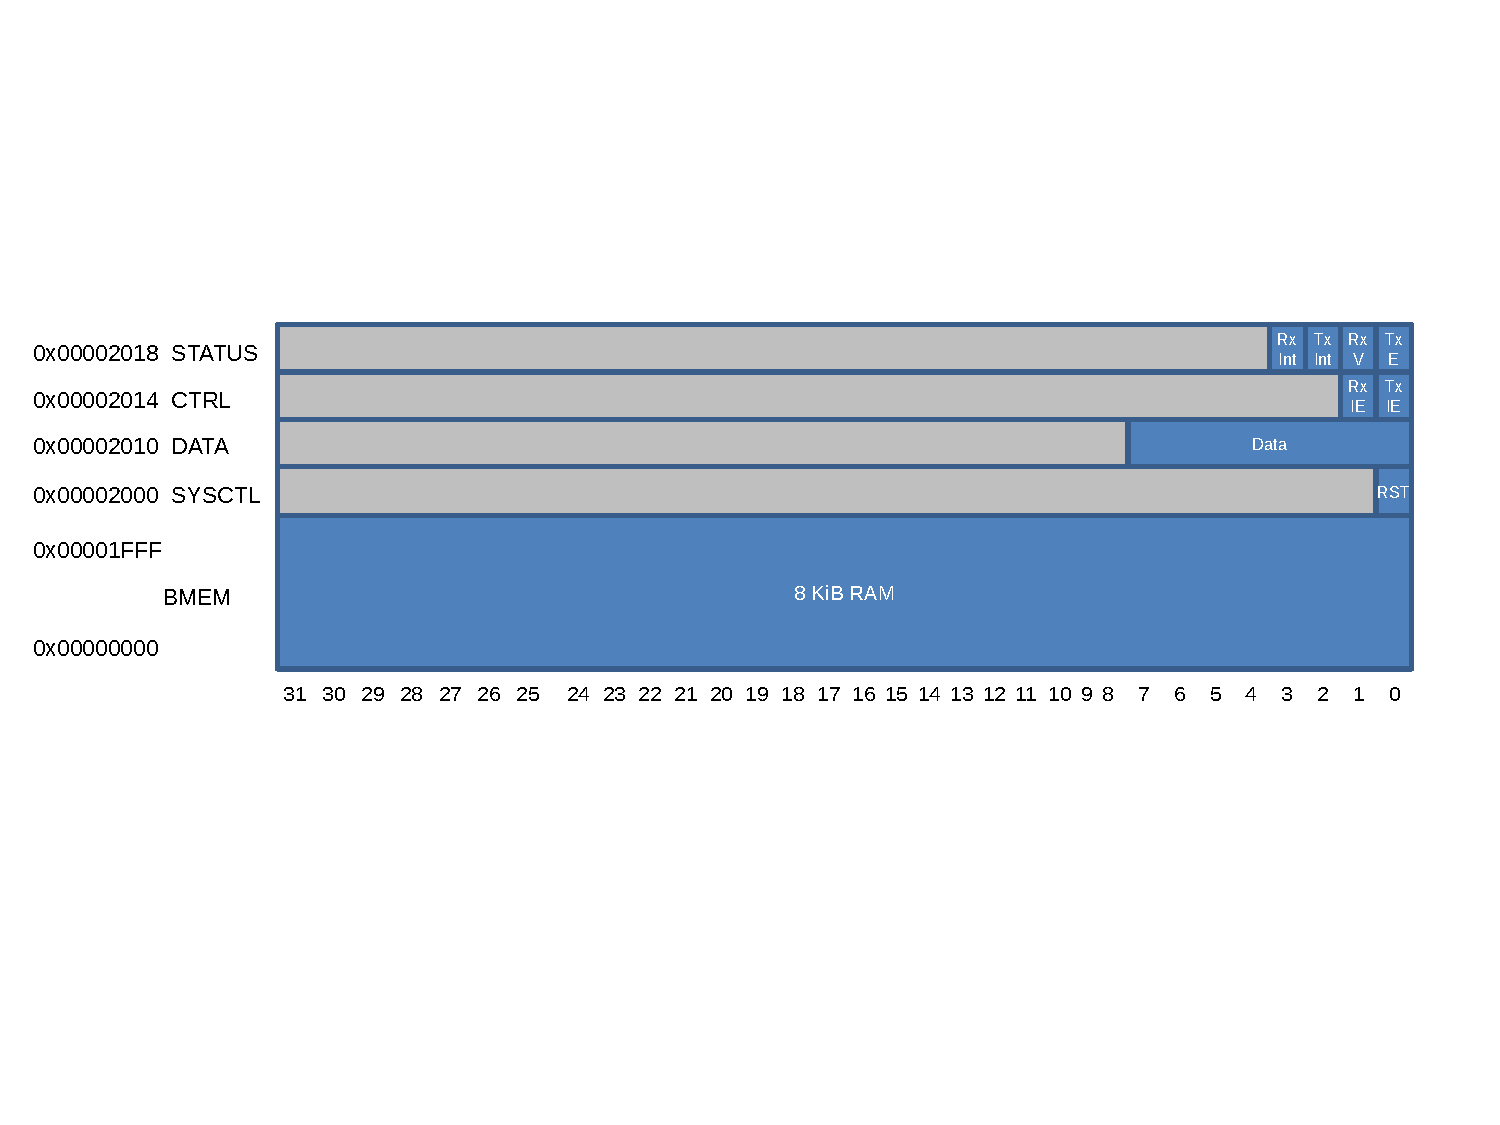
\includegraphics[width=\textwidth,clip=true,trim=0.5cm 7cm 0.5cm 5cm]{images/raggedstone1_ZPU.pdf}
	\end{frame}
	
	\begin{frame}{Grundideen}
		\begin{itemize}
			\item Aufteilung des Projekts in \textbf{unabhängige Module}, Bibliotheken und Anwendungen.
			\item Parsing der Intel HEX-Dateien und Kommunikation mit dem ZPU-Treiber in jeweils \textbf{eigene Bibliotheken}, die dann aus Anwendungen heraus genutzt werden.
			\item Die erstellten Bibliotheken sind \textbf{anwendungsunabhängig} und können später auch in Drittanwendungen verwendet werden.
		\end{itemize}
	\end{frame}

	\begin{frame}{Architekturentwurf (1)}
	\begin{center}
		\begin{tikzpicture}
	\usetikzlibrary{positioning}
	\tikzstyle{node}=[anchor=mid,text centered,minimum height=2em];
	\tikzstyle{app}=[draw,fill=green!50,rectangle]
	\tikzstyle{lib}=[draw,fill=yellow!50,rectangle]
	\tikzstyle{dri}=[draw,fill=red!50,rectangle]
				
	\draw [lib] (6,0.5) rectangle +(2,0.75) node [node,midway] {libzpu};
	\draw [lib] (4cm-2pt,0.5) rectangle +(2,0.75) node [node,midway] {libintelhex};
				
	\draw [dri] (-0.5,-0.5) rectangle +(8.5,-0.75) node [node,midway] {modzpu};
	\draw [app] (6,2) rectangle +(2,0.75) node [node,midway] {zpuio};
	\draw [app] (4cm-2pt,2) rectangle +(2,0.75) node [node,midway] {zpuload};
					
	\draw [dashed] (0,0) -- (8,0);
	\draw [->] (7,0.5) -- (7,-0.5);
	\draw [->] (7,2) -- (7,1.25);
	\draw [->] (5,2) -- (5,1.25);
	\draw [->] (5.5,2) -- (6.5,1.25);
				
	\node [anchor=west] at (-0.5, 2.375) {Userspace-Programme};
	\node [anchor=west] at (-0.5, 0.875) {Bibliotheken};
\end{tikzpicture}
	\end{center}
	\end{frame}
	
	\begin{frame}{Architekturentwurf (2)}
		\textbf{Kernel-Ebene:}
		\begin{itemize}
			\item Das Kernel-Modul \texttt{zpu} stellt \texttt{mmap}-, \texttt{read}-, \texttt{write}- und \texttt{ioctl}-\textbf{Systemaufrufe} zur Verfügung.
		\end{itemize}
		\textbf{Userspace-Bibliotheken:}
		\begin{itemize}
			\item Die Bibliothek \texttt{libzpu} stellt Funktionen zur Verfügung, um in Anwenderprogrammen vom Zugriff auf diese Systemaufrufe zu \textbf{abstrahieren}.
			\item Die Bibliothek \texttt{libintelhex} stellt Funktionen zum \textbf{Parsen von Intel HEX-Dateien} zur Verfügung.
		\end{itemize}
		\textbf{Userspace-Programme:}
		\begin{itemize}
			\item Das Programm \texttt{zpuio} kann \textbf{Eingaben} an die ZPU leiten und deren \textbf{Ausgabe} verarbeiten.
			\item Das Programm \texttt{zpuload} kann Intel HEX-Dateien lesen und \textbf{in die ZPU laden}.
		\end{itemize}
	\end{frame}
	
	\begin{frame}{Das \texttt{zpu}-Modul: Ein- und Ausgabe}
		\begin{center}
			\begin{tikzpicture}
	\usetikzlibrary{positioning}
	\tikzstyle{pci}=[draw,fill=green!50,rectangle]
	\tikzstyle{krn}=[draw,fill=yellow!50,rectangle]
				
	\draw [fill=green!20] (0,-0.5) rectangle +(8,2.5);
	\draw [fill=yellow!20] (0,2.5) rectangle +(8,2.5);
				
	%\draw [<->] (1.8,0.9) -- (5,0.9);
	%\draw [<->] (3.8,1.1) -- (5,1.1);
	\draw [<->,dotted] (6,1.5) -- (6,3);
			
	\draw [<->,dotted] (1,0.2) -- (1,-0.2) -- (6.1,-0.2) -- (6.1,0.5);
	\draw [<->,dotted] (3,0.2) -- (3,-0) -- (5.9,0) -- (5.9,0.5);
				
	\draw [<->,dotted] (3.2,4.3) -- (3.2,4.5) -- (5.9,4.5) -- (5.9,4);
	\draw [<->,dotted] (1.2,4.3) -- (1.2,4.7) -- (6.1,4.7) -- (6.1,4);
				
	%\draw [<->] (1.8,3.4) -- (5,3.4);
	%\draw [<->] (3.8,3.6) -- (5,3.6);
				
	\node [anchor=north east] at (8,-0.5) {PCI-Hardware};
	\node [anchor=south east] at (8, 5.0) {Kernel};
				
	\draw [pci] (0.2,0.2) rectangle +(1.6,1.6) node [align=left,midway] {Eingabe-\\FIFO\\(\texttt{stdin})};
	\draw [pci] (2.2,0.2) rectangle +(1.6,1.6) node [midway,align=left] {Ausgabe-\\FIFO\\(\texttt{stdout})};
					
	\draw [krn] (0.2,2.7) rectangle +(1.6,1.6) node [midway,align=left] {Eingabe-\\FIFO};
	\draw [krn] (2.2,2.7) rectangle +(1.6,1.6) node [midway,align=left] {Ausgabe-\\FIFO};
				
	\draw [->] (1,2.7) -- (1,1.8);
	\draw [<-] (3,2.7) -- (3,1.8);
				
	\draw [->] (1,5.5) -- (1,4.3);
	\draw [<-] (3,5.5) -- (3,4.3);
	\node [anchor=south] at (3,5.5) {\texttt{read()}};
	\node [anchor=south] at (1,5.5) {\texttt{write()}};
				
	\draw [pci] (5,0.5) rectangle +(2,1) node [align=left,midway] {Interrupt-\\Controller};
		\draw [krn] (5,3) rectangle +(2,1) node [midway] {IRQ-Handler};
\end{tikzpicture}
		\end{center}
	\end{frame}
	
	\begin{frame}{Das \texttt{zpu}-Modul: Ein- und Ausgabe}
	\begin{columns}
		\column{0.5\textwidth}
		\begin{itemize}
			\item Die \texttt{write}-Methode schreibt Daten in den Puffer (FIFO) des Moduls.
			\item Anschließend gibt sie den Empfangs-Interrupt (aus ZPU-Sicht) frei und legt sich (ggf.) schlafen.
			\item Der Empfangs-IR-Handler schreibt so viele Daten wie möglich in den \texttt{stdin}-Puffer der ZPU und weckt eventuell schlafende Schreibprozesse auf.
		\end{itemize}
		\column{0.5\textwidth}
		\begin{itemize}
			\item Die \texttt{read}-Methode liest Daten aus dem Puffer (FIFO) des Moduls und gibt ggf. den Sende-IR-Handler wieder frei.
			\item Sollte der Puffer leer sein, legt sich die \texttt{read}-Methode (ggf.) schlafen.
			\item Der Sende-IR-Handler (aus ZPU-Sicht) liest so viele Daten wie möglich aus dem \texttt{stdout}-Puffer der ZPU in den Puffer des Moduls und weckt eventuell schlafende Leseprozesse auf.
		\end{itemize}
	\end{columns}
	\end{frame}
	
	\begin{frame}[fragile]{Ein- und Ausgabe}
	\begin{lstlisting}[language=C,basicstyle=\footnotesize\ttfamily]
	static ssize_t zpu_chr_write (struct file *filep,
	  const char __user *data, size_t count, loff_t *offset) {
  fifo_t       *f = &(zpu_io_stdin);
  unsigned int  n;

  if (FIFO_FULL(f)) {
    ZPU_ENABLE_STDIN_IR();

    if (filep->f_flags & O_NONBLOCK)
      return -EAGAIN;
    else if (wait_event_interruptible(f->queue, FIFO_NOT_FULL(f)) != 0)
      return -EINTR;
  }

  /* Kopieren mit copy_from_user */

  f->count = f->count + n;
  ZPU_ENABLE_STDIN_IR();

  return n;
}
	\end{lstlisting}
	\end{frame}
	
	\begin{frame}{Vorgehen}
		\begin{itemize}
			\item Testgetriebene Entwicklung der Bibliotheken und Anwenderprogramme (z.B. mit CUnit\footnote{\url{http://cunit.sourceforge.net/}})
			\item Erstellung portabler Build-Skripte mit \texttt{autoscan} und \texttt{autoconf}.\footnote{\url{http://www.gnu.org/software/autoconf/}}
			\item Git\footnote{\url{http://git-scm.com/}} als Versionskontrollsystem. Zentrale Verwaltung auf Github, transparente Entwicklung. Organisation der erstellten Komponenten in unabhängigen Git-Repositories.
		\end{itemize}
	\end{frame}
	
	\section{Die libintelhex-Bibliothek}
	
	\begin{frame}[fragile]{Das Intel HEX-Format}
		\begin{lstlisting}[frame=single]
			:1000000000000000000000000000000000000000F0
:0400100000000000EC
:100400000B0B0B98B02D0B0B0B8880040000000029
:1004100000000000000000000000000000000000DC
// ...
:1010E200000008D9000008D9000008D9000008D97A
:1010F200000008D9000008D9000008D9000008D96A
:0C110200000008D9000008D9000008D93E
:0400000300000400F5
:00000001FF
		\end{lstlisting}
	\end{frame}
	
	\begin{frame}{Die \texttt{libintelhex}-Bibliotek: API}
		Die \texttt{libintelhex}-Bibliothek stellt Methoden zum Einlesen von Intel HEX-Dateien zur Verfügung.
		
		\begin{description}[style=nextline,font=\ttfamily\bfseries]
			\item[struct *ihex\_recordset ihex\_rs\_from\_file(char* filename)]
			Liest Binärdaten aus einer Dateieingabe ein.
			\item[struct *ihex\_recordset ihex\_rs\_from\_str(char* input)]
			Liest Binärdaten aus einer Zeichenkette ein.
			\item[int ihex\_mem\_copy(struct *ihex\_records rec, void* dst, uint\_t l, ihex\_width\_t w, ihex\_byteorder\_t o)]
			Kopiert Daten an eine beliebige (durch \texttt{dst}) angegebene Position. \texttt{l} ist die Größe des Ziel-Speicherbereichs. \texttt{w} gibt die Art des Speicherzugriffs an (bei der ZPU 32 Bit) und \texttt{o} die Byte-Reihenfolge.
		\end{description}
	\end{frame}
	
	\begin{frame}[fragile]{Die \texttt{libintelhex}-Bibliotek: Datenstrukturen}
		\begin{lstlisting}[language=C]
typedef struct ihex_record {
    unsigned int ihr_length;
    ihex_rtype_t ihr_type;     // enum {...}
    ihex_addr_t  ihr_address;  // uint16
    ihex_rdata_t ihr_data;     // uint8*
    ihex_rchks_t ihr_checksum; // uint8
} ihex_record_t;

typedef struct ihex_recordset {
    unsigned int   ihrs_count;
    ihex_record_t* ihrs_record;
} ihex_records_t;
		\end{lstlisting}
	\end{frame}
	
	\begin{frame}{Die \texttt{libintelhex}-Bibliothek: Datenstrukturen}
	\begin{center}
		\begin{tikzpicture}
	\usetikzlibrary{arrows}
	\tikzstyle{attr}=[midway,text width=3.3cm,text height=0.3cm]
	\tikzstyle{green}=[fill=green!20]
	\tikzstyle{yellow}=[fill=yellow!20]	
			
	\draw [fill=green!50] (0,0) rectangle +(3.5,0.5) node [attr] {\texttt{ihex\_recordset\_t}};
	\draw [green] (0,-0.5) rectangle +(3.5,0.5) node [attr] {\texttt{ihrs\_count} = 2};
	\draw [green] (0,-1) rectangle +(3.5,0.5) node [attr] {\texttt{ihrs\_records} = };
			
	\draw [fill=yellow!50] (0,-2) rectangle +(3.5,0.5) node [attr] {\texttt{ihex\_record\_t}};
	\draw [yellow] (0,-2.5) rectangle +(3.5,0.5) node [attr] {\texttt{ihr\_length} = 4};
	\draw [yellow] (0,-3) rectangle +(3.5,0.5) node [attr] {\texttt{ihex\_type} = 0x00};
	\draw [yellow] (0,-3.5) rectangle +(3.5,0.5) node [attr] {\texttt{ihex\_addr} = 0x00};
	\draw [yellow] (0,-4) rectangle +(3.5,0.5) node [attr] {\texttt{ihex\_data} = };
			
	\draw [fill=yellow!50] (3.5,-2) rectangle +(3.5,0.5) node [attr] {\texttt{ihex\_record\_t}};
	\draw [yellow] (3.5,-2.5) rectangle +(3.5,0.5) node [attr] {\texttt{ihr\_length} = 6};
	\draw [yellow] (3.5,-3) rectangle +(3.5,0.5) node [attr] {\texttt{ihex\_type} = 0x00};
	\draw [yellow] (3.5,-3.5) rectangle +(3.5,0.5) node [attr] {\texttt{ihex\_addr} = 0x04};
	\draw [yellow] (3.5,-4) rectangle +(3.5,0.5) node [attr] {\texttt{ihex\_data} = };
			
	\draw[*->] (3,-0.7) -- (3,-1.5);
	\draw[*->] (2.5,-3.7) -- (2.5,-4.5) -- (0.75/2, -4.5) -- (0.75/2,-5);
	\draw[*->] (6,-3.7) -- (6,-4.5) -- (3.5+0.75/2, -4.5) -- (3.5+0.75/2,-5);
			
	\foreach \x in {0,0.75,1.5,2.25}{
		\draw (\x, -5.5) rectangle +(0.75,0.5) node [attr,text width=0.7cm] {0x00};
	};
			
	\foreach \x in {3.5,4.25,5,5.75,6.5,7.25}{
		\draw (\x, -5.5) rectangle +(0.75,0.5) node [attr,text width=0.7cm] {0x00};
	};
\end{tikzpicture}
		\end{center}
	\end{frame}
	
	\begin{frame}[fragile]{Anwendungsbeispiel}
		\begin{lstlisting}[language=C,breaklines=true,numbers=left]
#include <stdlib.h>
#include <cintelhex.h>

int main()
{
  ihex_recordset_t* r = ihex_rs_from_file("in.hex");
  void*             d = malloc(8192);
	
  if (r != NULL)
  {
    return ihex_mem_copy(r, d, 8192, IHEX_WIDTH_32BIT, IHEX_ORDER_BIGENDIAN);
  }
  return ihex_errno();
}
		\end{lstlisting}
	\end{frame}
	
	\begin{frame}
		Die \textbf{cIntelHEX}-Bibliothek ist \textbf{Open Source} (GNU LGPL):
		
		\begin{itemize}
			\item \url{https://github.com/martin-helmich/libcintelhex}
		\end{itemize}
	\end{frame}
	
	\section{Die libzpu-Bibliothek}
	
	\begin{frame}{Die \texttt{libzpu}-Bibliothek}
	
		Die \texttt{libzpu}-Bibliothek soll im Userspace stark abstrahierte Methoden zur Steuerung der ZPU zur Verfügung stellen. Unterstützte Funktionen sind das \textbf{Laden neuer Programme} und \textbf{Ein- und Ausgabebehandlung}.
		
		Die Methoden werden in \texttt{zpu.h} definiert.
		
		\begin{description}[style=nextline,font=\ttfamily\bfseries]
			\item[int zpu\_from\_hexfile(char* filename)] Lädt ein ZPU-Programm aus einer Intel HEX-Datei in die ZPU. Liefert im Erfolgsfall \texttt{0} zurück. Stoppt die ZPU implizit und startet sie anschließend wieder.
			\item[int zpu\_stop()]
			Versetzt die ZPU in den Reset-Modus.
			\item[int zpu\_start()]
			Startet die ZPU wieder.
		\end{description}
	\end{frame}
	
	\subsection{Userspace-Programme}
	
	\begin{frame}[fragile]{Userspace-Programme}
		\begin{lstlisting}[numbers=left,frame=single]
			> zpuload input.hex
			Loading program "input.hex"...
			Loaded program.
		\end{lstlisting}
		
		\begin{lstlisting}[numbers=left,frame=single]
			> zpuio
			output (11) > Hallo Welt!
			input > Hallo auch.
			output (11) > HAllo Auch.
			intput >
		\end{lstlisting}
	\end{frame}
	
	\begin{frame}{Ausblick}
		\begin{itemize}
			\item Gerätedateien automatisch bei Registrierung des Geräts erstellen (geht mit \textbf{udev}).
			\item Beim Booten automatisch eine Firmware aus dem Dateisystem in das Gerät laden (z.B. über eine \textbf{udev-Regel}, die zpuload aufruft).
		\end{itemize}
		\vspace{1cm}
		\begin{center}
			\huge Fragen?
		\end{center}
	\end{frame}
\end{document}
